\documentclass[11pt]{article}
\usepackage{standalone}
\usepackage[utf8]{inputenc}
\usepackage{mathtools}
\usepackage{gensymb}
\usepackage{amsmath}
\usepackage{amssymb}
\usepackage{tikz}
\usepackage{gensymb}
\usepackage{esvect}
\usetikzlibrary{arrows}

\begin{document}
\section*{Problème}
Le personnel de la tour de contrôle d'un aéroport repère un OVNI. À 11 h 02, il se trouve à une distance horizontale de $2\text{ km}$ selon une orientation de $30\degree$ nord par rapport à l'est à une altitude de $1200\text{ m}$. À 11h 15, sa position est $1\text{ km}$ à $45\degree$ sud par rapport à l'est à une altitude de $800\text{ m}$. Décrivez le vecteur déplacement de l'OVNI entre ces deux positions.\cite{problem}

\section*{Résolution}
Soit $A$ et $B$ les positions avant et après de l'OVNI respectivement. Les vecteurs qui commencent à l'origine et qui se rendent juste qu'à ces deux points sont $\vv{OA}$ et $\vv{OB}$ respectivement. On cherche le vecteur déplacement de $A$ à $B$, tel que $\vv{AB}=\vv{OB}-\vv{OA}$. Voici un schéma qui traduit les coordonnées polaires de l'énoncé en composantes. Toutes les mesures sont en $km$.
\begin{center}
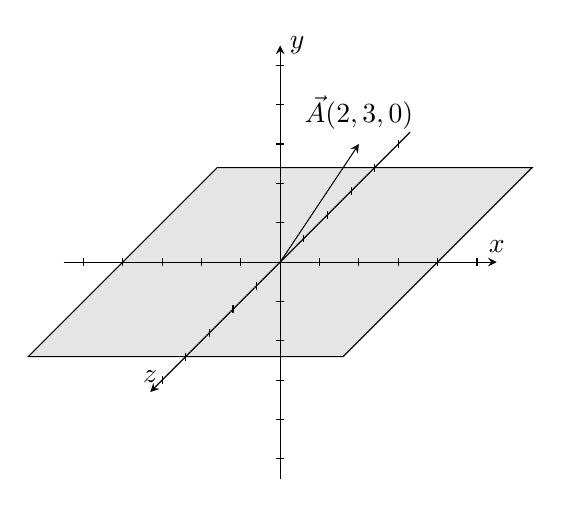
\begin{tikzpicture}[x=0.5cm,y=0.5cm,z=0.3cm,>=stealth]
\coordinate (O) at (0,0,0);
\coordinate (A) at (2,3,0);
\coordinate (P1) at (-5,-5,0);
\coordinate (P2) at (-5, 5,0);
\coordinate (P3) at ( 5, 5,0);
\coordinate (P4) at ( 5,-5,0);
% The axes
\draw[->] (xyz cs:x=-5.5) -- (xyz cs:x= 5.5) node[above] {$x$};
\draw[->] (xyz cs:y=-5.5) -- (xyz cs:y= 5.5) node[right] {$y$};
\draw[->] (xyz cs:z= 5.5) -- (xyz cs:z=-5.5) node[above] {$z$};

% The thin ticks
\foreach \coo in {-5,-4,...,5} {
  \draw (\coo,-1.5pt) -- (\coo,1.5pt);
  \draw (-1.5pt,\coo) -- (1.5pt,\coo);
  \draw (xyz cs:y=-0.10pt,z=\coo) -- (xyz cs:y=0.10pt,z=\coo);
}

% The vector
\draw[->] (O) -- (A);
\node[inner sep=1.5pt,label={above:$\vec{A}(2, 3, 0)$}] at (A) {};

% The plane
\draw[fill=black, fill opacity=0.1] 
	(xyz cs:x=-4,z=-4) -- (xyz cs:x=-4,z= 4) -- 
	(xyz cs:x= 4,z= 4) -- (xyz cs:x= 4,z=-4) -- cycle;
\end{tikzpicture}
\end{center}
\pagebreak

Il suffit de soustraire les composantes des deux vecteurs :
\begin{equation*}
\begin{split}
\vv{AB}&=\vv{OB}-\vv{OA}\\
       &=(1\cos315\degree\vec{i}+1\cos315\degree\vec{j}+0.80\vec{k})-(2\cos30\degree\vec{i}+2\cos30\degree\vec{j}+1.20\vec{k})\\
       &\approx(0,71\vec{i}-0.71\vec{j}+0.80\vec{k})-(1.73\vec{i}+1.00\vec{j}+1.20\vec{k})\\
       &=(-1.02\vec{i}-1.71\vec{j}+0.40\vec{k})\text{ km}
\end{split}
\end{equation*}

\section*{Bibliographie}
\bibliographystyle{plain}
\renewcommand{\section}[2]{}
\bibliography{bibliography}
\end{document}
